\documentclass[11pt]{report}
\usepackage{amsmath, bm, xcolor, graphicx, listings}
\usepackage{courier} %for listings
\usepackage{caption}
\usepackage{subcaption}
\lstset{basicstyle=\footnotesize\ttfamily,breaklines=true} %listing font settings
%\lstset{framextopmargin=50pt} %listing font settings
\usepackage[english]{babel}
\setlength\parindent{0pt} %remove indentation in new paragraphs

\begin{document}

\title{Poisson Solver (2D)}
\author{Nikos Tryfonidis}
\date{2015}
\maketitle

\begin{abstract}
The current report summarizes the structure, use and results of a two-dimensional Poisson solver, 
created for the purpose of being integrated into a 2D Particle-In-Cell (PIC) code. After a brief introduction 
regarding the numerical solution of the 2D Poisson PDE in chapter 1, the structure of the code will be 
described in chapter 2. Verification of the code will be given in chapter 3, through a number of test cases. 
Finally, the performance of the code will be discussed in chapter 4.
\end{abstract}

\tableofcontents

\chapter{2D Poisson Equation: Numerical Solution}
The Poisson Equation and the associated boundary conditions form what is generally known as a 
\emph{Poisson Problem}: 

\begin{equation}
\nabla ^2 u = u_{xx} + u_{yy} = f(x,y)
\end{equation}

The Poisson Problem is one of the most well-known Elliptic Partial Differential Equations (PDE). A brief description of the numerical method followed in the code will be given here. Detailed analysis of the Poisson PDE and other methods can be found in most numerical analysis textbooks (for example [1]).

\section{The Finite Difference Scheme}
The 5-point stencil discretization scheme is followed. A uniform Cartesian grid is used, where each point $x_i, y_j$ describes a point in 2D space, with $x_i = i\Delta x$ and $y_j = j\Delta y$. We assume that $0 \leq x \leq 1$ and $0 \leq y \leq 1$ for simplicity. Replacing the derivatives $u_{xx}$ and $u_{yy}$ in (1.1) with centered finite difference schemes, we end up with the following discretization scheme:

\begin{equation}
\frac{1}{(\Delta x)^2}(u_{i-1,j} -2u_{i,j} + u_{i+1,j}) + 
\frac{1}{(\Delta y)^2}(u_{i,j-1} -2u_{i,j} + u_{i,j+1}) = f_{i,j}
\end{equation}

Assuming that $\Delta x = \Delta y = h$, we get the simple finite difference scheme

\begin{equation}
u_{i-1,j} + u_{i+1,j} + u_{i,j-1} + u_{i,j+1} - 4u_{i,j} = h^2 f_{i,j}
\end{equation}

For a grid of $N \times N$ points in total, this scheme gives a linear system of $(N-2) \times (N-2)$ equations for the $(N-2) \times (N-2)$ unknowns (the excluded values are the boundaries, which are considered known). As an example to illustrate the system of equations, suppose we have a $5 \times 5$ grid of points, including boundaries, that represent our 2D space. 

\begin{figure}[h]
\centering
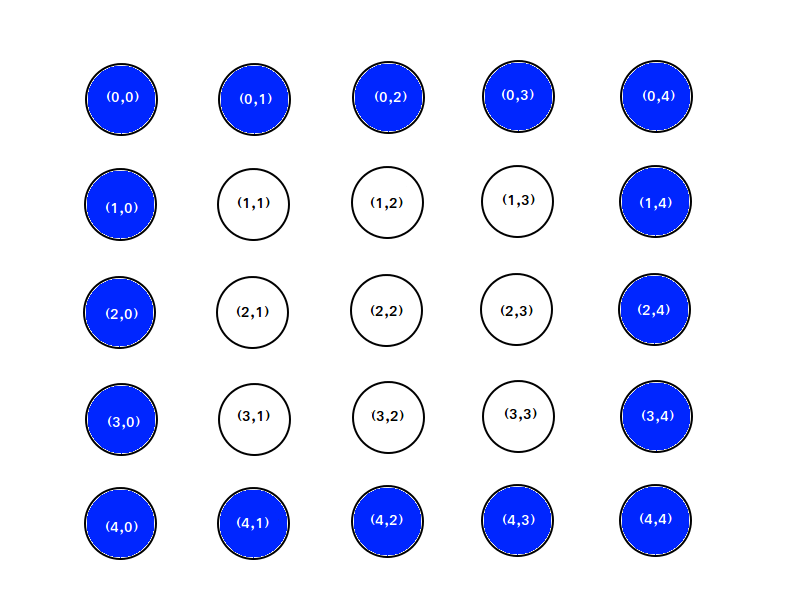
\includegraphics[scale=0.35]{images/grid}
\caption{A $5 \times 5$ two-dimensional grid. 
Boundary points, for which the solution is known, are shown in blue. }
\label{fig:Space grid 5x5}
\end{figure}

Applying the finite difference scheme (1.3) to each inner grid point $u_{i,j}$ leads us to a system of $(5-2) \times (5-2) = 9$ equations:

\begin{subequations}
\begin{align}
\bm{u_{1,1}}: 
\quad  & \textcolor{blue}{u_{0,1}} + u_{2,1} + \textcolor{blue}{u_{1,0}} + u_{1,2} - 4u_{1,1} = h^2 f_{1,1} \\
\bm{u_{1,2}}: 
\quad  & \textcolor{blue}{u_{0,2}} + u_{2,2} + u_{1,1} + u_{1,3} - 4u_{1,2} = h^2 f_{1,2} \\
\bm{u_{1,3}}: 
\quad  & \textcolor{blue}{u_{0,3}} + u_{2,3} + u_{1,2} + \textcolor{blue}{u_{1,4}} - 4u_{1,3} = h^2 f_{1,3} \\
\bm{u_{2,1}}: 
\quad  & u_{1,1} + u_{3,1} + \textcolor{blue}{u_{2,0}} + u_{2,2} - 4u_{2,1} = h^2 f_{2,1} \\
\bm{u_{2,2}}:
\quad  & u_{1,2} + u_{3,2} + u_{2,1} + u_{2,3} - 4u_{2,2} = h^2 f_{2,2} \\
\bm{u_{2,3}}: 
\quad  & u_{1,3} + u_{3,3} + u_{2,2} + \textcolor{blue}{u_{2,4}} - 4u_{2,3} = h^2 f_{2,3} \\
\bm{u_{3,1}}: 
\quad  & u_{2,1} + \textcolor{blue}{u_{4,1}} + \textcolor{blue}{u_{3,0}} + u_{3,2} - 4u_{3,1} = h^2 f_{3,1} \\
\bm{u_{3,2}}: 
\quad  & u_{2,2} + \textcolor{blue}{u_{4,2}} + u_{3,1} + u_{3,3} - 4u_{3,2} = h^2 f_{3,2} \\
\bm{u_{3,3}}: 
\quad  & u_{2,3} + \textcolor{blue}{u_{4,3}} + u_{3,2} + \textcolor{blue}{u_{3,4}} - 4u_{3,3} = h^2 f_{3,3}
\end{align}
\end{subequations}

\vspace{0.3cm}
We have arranged the equations row-wise, grouping elements with the same row number ($i$ index) together. We 
also see the boundary grid points in blue. These are considered to be known from the given boundary conditions.
\newline

We can now present the linear system of equations in matrix form,

\begin{equation}
\overleftrightarrow{\textbf{A}} \cdot \overrightarrow{\textbf{u}} = \overrightarrow{\textbf{b}},
\end{equation}

\vspace{0.3cm}

where $\overleftrightarrow{\textbf{A}}$ is the matrix equation, $\overrightarrow{\textbf{u}}$ is the vector of unknowns and $\overrightarrow{\textbf{b}}$ is the right-hand-side of the system of equations. Note that we will move the known boundary grid points to the right-hand-side of the matrix equation (again, shown in blue). The resulting matrix equation is

%%%Matrix with labels (uses parentheses): 
\begin{equation*}
\let\quad\thinspace
\bordermatrix{\text{}& \bm{u_{1,1}} & \bm{u_{1,2}} & \bm{u_{1,3}} & \bm{u_{2,1}} & \bm{u_{2,2}} & \bm{u_{2,3}} & \bm{u_{3,1}} & \bm{u_{3,2}} & \bm{u_{3,3}} \cr
   & -4 & 1 & 0 & 1 & 0 & 0 & 0 & 0 & 0  \cr
   & 1 & -4 & 1 & 0 & 1 & 0 & 0 & 0 & 0  \cr
   & 0 & 1 & -4 & 0 & 0 & 1 & 0 & 0 & 0  \cr 
   & 1 & 0 & 0 & -4 & 1 & 0 & 1 & 0 & 0  \cr
   & 0 & 1 & 0 & 1 & -4 & 1 & 0 & 1 & 0  \cr
   & 0 & 0 & 1 & 0 & 1 & -4 & 0 & 0 & 1  \cr
   & 0 & 0 & 0 & 1 & 0 & 0 & -4 & 1 & 0  \cr
   & 0 & 0 & 0 & 0 & 1 & 0 & 1 & -4 & 1  \cr
   & 0 & 0 & 0 & 0 & 0 & 1 & 0 & 1 & -4 
    }
\cdot
\begin{pmatrix}
u_{1,1} \\ u_{1,2} \\ u_{1,3} \\ u_{2,1} \\ u_{2,2} \\ u_{2,3} \\ u_{3,1} \\ u_{3,2} \\ u_{3,3}
\end{pmatrix}
=
\begin{pmatrix}
h^2f_{1,1} + \textcolor{blue}{u_{0,1}} + \textcolor{blue}{u_{1,0}} \\ 
h^2f_{1,2} + \textcolor{blue}{u_{0,2}} \\ 
h^2f_{1,3} + \textcolor{blue}{u_{0,3}} + \textcolor{blue}{u_{1,4}} \\
h^2f_{2,1} + \textcolor{blue}{u_{2,0}} \\
h^2f_{2,2} \\
h^2f_{2,3} + \textcolor{blue}{u_{2,4}} \\
h^2f_{3,1} + \textcolor{blue}{u_{4,1}} + \textcolor{blue}{u_{3,0}} \\
h^2f_{3,2} + \textcolor{blue}{u_{3,2}} + \textcolor{blue}{u_{4,2}} \\
h^2f_{3,3} + \textcolor{blue}{u_{4,3}} + \textcolor{blue}{u_{3,4}}
\end{pmatrix}
\end{equation*}
\vspace{0.75cm}

We see that the resulting $\overleftrightarrow{\textbf{A}}$ matrix is block-tridiagonal:

\begin{equation}
\overleftrightarrow{\textbf{A}} = 
\begin{pmatrix}
\bm{T} & \bm{I} & \bm{0} \\
\bm{I} & \bm{T} & \bm{I} \\
\bm{0} & \bm{I} & \bm{T}
\end{pmatrix}
\end{equation}
\vspace{0.5cm}
\begin{equation}
\bm{T} =
\begin{pmatrix}
-4 & 1 & 0 \\
1 & -4 & 0 \\
0 & 1 & -4
\end{pmatrix}
, \quad
\bm{I} =
\begin{pmatrix}
1 & 0 & 0 \\
0 & 1 & 0 \\
0 & 0 & 1
\end{pmatrix}
, \quad
\bm{0} =
\begin{pmatrix}
0 & 0 & 0 \\
0 & 0 & 0 \\
0 & 0 & 0
\end{pmatrix}
\end{equation}

\vspace{0.5cm}

This linear system of equations can be solved with a variety of methods (direct, iterative etc). Our focus will be on iterative methods.

\section{Error and Stability}
We will not go into the details of error and stability analysis in this report, since these are well-known 
and can be found in most relevant texts (e.g. [1]). We should simply keep in mind that the local truncation error of the 5-point stencil finite difference scheme we are using is $O(h^2)$ and that the method is stable, so the global error of the method is also $O(h^2)$. In case we do not assume $\Delta x = \Delta y = h$, this 
simply means that the error is $O\left( (\Delta x)^2, (\Delta y)^2 \right)$.

\chapter{The Code}
In this chapter, the structure and use of the code will be described. The project has been arranged into 
separate directories. The source code is in "src", with corresponding header files in "headers", one for each 
.c source file (other than "main.c"). Object files (".o") are automatically placed into the "obj" directory by the makefile. Output files are also placed into the "output" directory. The python visualization script used 
for plotting the output is also in "output". Finally, "documentation" contains the current report.

In the following sections, we will briefly go through instructions on how to use the code, and we will review its structure.

\section{Compilation and Execution}
The code does not contain any external libraries and should compile without problems on any linux system with a C compiler. To compile, go to the central directory of the project, where the makefile is located, and type "make". This will create the executable file in the same directory, with object files in "obj". To delete the executable and the object files, type "make clean".

To run, simply run the executable from the command line, giving two arguments (number of grid points in dimensions X and Y, respectively). For example, the following will run the program with 101 grid points in X and Y:

\begin{lstlisting}
./poisson2D 101 101
\end{lstlisting}

\section{Code Structure}
Here we will briefly go through the code structure, by explaining the work done by each of the source files. 

\begin{description}
  \item[main.c] The main file simply wraps all pieces of the program together and can be seen as a program outline. First it reads the command line arguments and it allocates the required memory. Then, it sets up the problem, by setting the appropriate Boundary Conditions and right-hand-side function f(x,y) (see "setup.c").
  \item[io.c] Contains functions that read command line arguments and write file output.
  \item[setup.c] Contains functions that set boundary conditions and the right-hand-side function. This is where the user can specify the Poisson problem he/she wants to solve. \emph{Boundary conditions} can be set for each one of the four boundaries separately, by the $"setBoundaries2D"$ function. The RHS function is set by $"setRHS2D"$.
  \item[memory.c] Contains the $"array2D_contiguous"$ function, that dynamically allocates a two-dimensional array of doubles, contiguous in memory. Also contains the $"free_array2D_contiguous"$ function, that frees memory allocated by the previous function.
  \item[poisson2D.c] The solver function. It iterates the solution for the appropriate number of iterations, until the desired accuracy is reached (or a maximum number of iterations is done). The iteration method of choice is passed into the function as an argument (function pointer). Error tolerance, maximum iterations, iterations per residual check are all set in this function. Also contains the residual calculation function.
  \item[iterative.c] Contains the different iterative methods that may be used, and that are called by $"solvePoisson2D"$. Currently, the Jacobi, Gauss-Seidel and Successive Overrelaxation methods have been implemented.
\end{description}

The space dimensions $(x_0, x_L), (y_0, y_L)$ are set in \emph{definitions.h}, inside the \emph{headers} directory.

\section{Data Structures}
The main data structure used is a two-dimensional array of doubles, that represents the discretized space grid. The dimensions of the grid are given from the command line arguments the user provides. Memory for the 2D array is allocated by the $"array2D_contiguous"$ function in \emph{memory.c}.
\newline

Also, another two-dimensional array of the same dimensions is the right-hand-side function (RHS) of the Poisson Equation, $f(x,y)$. Memory for the RHS function is allocated in the same way as for the grid. The values of RHS for each grid point is set by the $"setRHS2D"$ function in \emph{setup.c}.

\section{Solving a Poisson Problem}
To solve a given Poisson problem, the user must perform the following actions:

\begin{enumerate}
  \item Set Boundary Conditions in \emph{setBoundaries2D.c} (setup.c).
  \item Set the RHS function of the Poisson problem in \emph{setRHS2D.c} (setup.c).
  \item Choose the desired iterative method in main function (main.c).
  \item Compile the program by typing "make" in the main directory (where the makefile is located).
  \item Run the executable with the desired number of grid points in each of the two dimensions.
\end{enumerate}

\section{Output}
Output is written in the "output" directory. Two output files are written:

\begin{description}
  \item[output.txt] Contains the 2D solution grid.
  \item[gridData.txt] Contains grid data $\left( (x_0, x_L), (y_0, y_L) \right) $, step sizes ($dx, dy$) and number of grid points in each dimension ($N_x, N_y$). Data from this file is read by the visualization python script in the same folder, in order to create a plot of the results.
\end{description}

The solution is visualized by the python script \emph{visualize.py}, in the output directory.
The script requires \emph{numpy} and \emph{matplotlib}, two well-known packages for scientific computing in Python.

These can be easily installed in any Linux system, for example in Ubuntu:

\begin{lstlisting}
sudo apt-get install python-numpy python-matplotlib
\end{lstlisting}

This python script reads grid meta-data from \emph{gridData.txt} and the solution from \emph{output.txt} and creates a 3D plot of the solution.

To create the plot, the user must simply run the script by typing:

\begin{lstlisting}
python visualize.py
\end{lstlisting}

\chapter{Verification}
In this chapter we will verify the correctness of the 2D Poisson solver, through three basic examples that have known analytic solutions. By comparing the numerical solution with the analytic one, we will show that the solver produces correct results.
\newline

Each example has detailed instructions on how to set up the Poisson problem studied, so the following sections can also be used as examples on how to use the code. The \emph{Gauss-Seidel} iterative method was chosen for these examples, with a tolerance of $\Delta x^2$ for the residual check.
\newline

For the following examples, the domain was chosen to be $0 \leq x,y \leq 1$, which is set in \emph{headers/definitions.h} as follows:

\begin{lstlisting}
#define X0 0.0
#define XL 1.0
#define Y0 0.0
#define YL 1.0
\end{lstlisting}

We also used 101 grid points for each dimension, dividing each dimension into $(101 - 1)$ pieces, so that 
\begin{equation}
\Delta x = \Delta y = (Length) / (101 - 1) = 1.0 / 100 = 0.01
\end{equation}
\newpage

\section{Zero RHS (Laplace Equation)}
In this problem, we will solve a Poisson problem with no right-hand-side function. Let us assume that the (known) solution $u(x,y)$ is 

\begin{equation}
u(x,y) = 3x + 4y
\end{equation}

The corresponding Poisson problem is then

\begin{subequations}
\begin{align}
\nabla ^2 u = &u_{xx} + u_{yy} = 0 \\
u(x,0) = 3x \quad \quad \quad & \quad \quad \quad u(x,y_L) = 3x + 4y_L \\
u(0,y) = 4y \quad \quad \quad & \quad \quad \quad u(x_L,y) = 3x_L + 4y
\end{align}
\end{subequations}

Equation $(3.2a)$, along with boundary conditions $(3.2b)$ and $(3.2c)$ are also known as a Laplace problem, a special case of the Poisson problem with a zero right-hand-side function. We will now solve this Poisson problem and compare the numerical solution with the analytic $(3.1)$.

\subsection{Setting Up The Problem}
As explained in paragraph \emph{2.4}, the functions that are used to set up the desired Poisson problem are in \emph{setup.c}. Boundary conditions are given by the known solution \emph{(3.1)}, while the RHS function is zero for this problem. 
\newline

We set the Boundary Conditions:

\begin{lstlisting}
double fBC(double x, double y) 
{
    return 3.0*x + 4.0*y;
}
\end{lstlisting}

and the RHS function:

\begin{lstlisting}
double f(double x, double y) 
{
    return 0.0;
}
\end{lstlisting}

\subsection{Running the Solver}
After we set up the problem as shown, we compile the program by typing "make" in the main project directory. 
Then, we simply run the program by specifying how many grid points we want to divide our domain into. 
\newline 

To specify 101 grid points for $x$ and $y$, we run the executables as follows:

\begin{lstlisting}
./poisson2D 101 101
\end{lstlisting}

Once the program has finished, output is ready in \emph{output/output.txt}. We can plot the solution by running the python script \emph{visualize.py}, which will create a 3D surface plot of our solution. In the next figure, the analytic and numerical solutions are shown side by side for comparison:

\begin{figure}[h!]
\centering
\begin{subfigure}{0.5\textwidth}
  \centering
  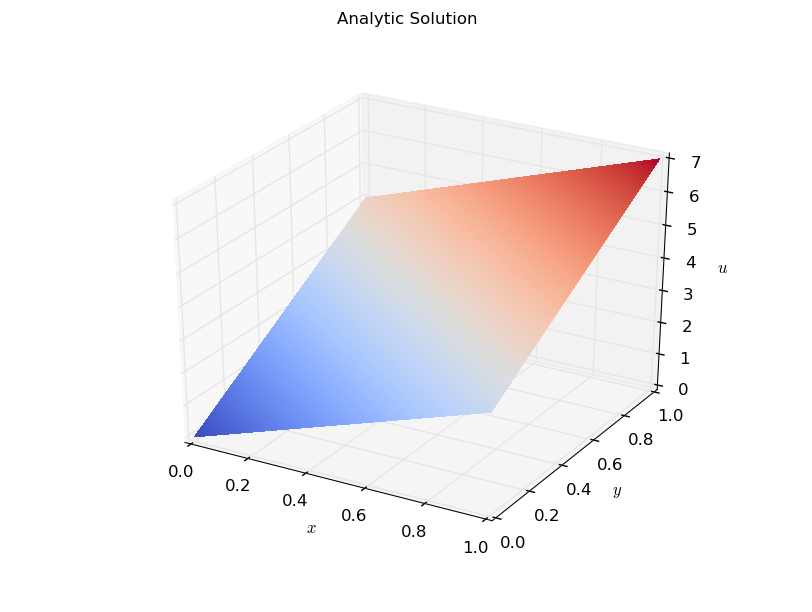
\includegraphics[width=1.0\linewidth]{images/example1_analytic}
  \caption{Analytic solution}
  \label{fig:sub1}
\end{subfigure}%
\begin{subfigure}{0.5\textwidth}
  \centering
  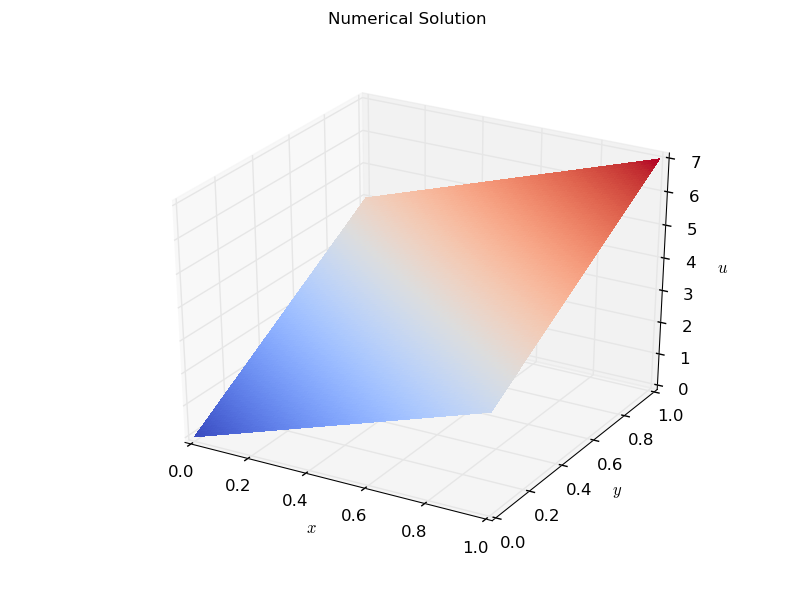
\includegraphics[width=1.0\linewidth]{images/example1_numerical}
  \caption{Numerical solution}
  \label{fig:sub2}
\end{subfigure}
\begin{subfigure}{0.6\textwidth}
  \centering
  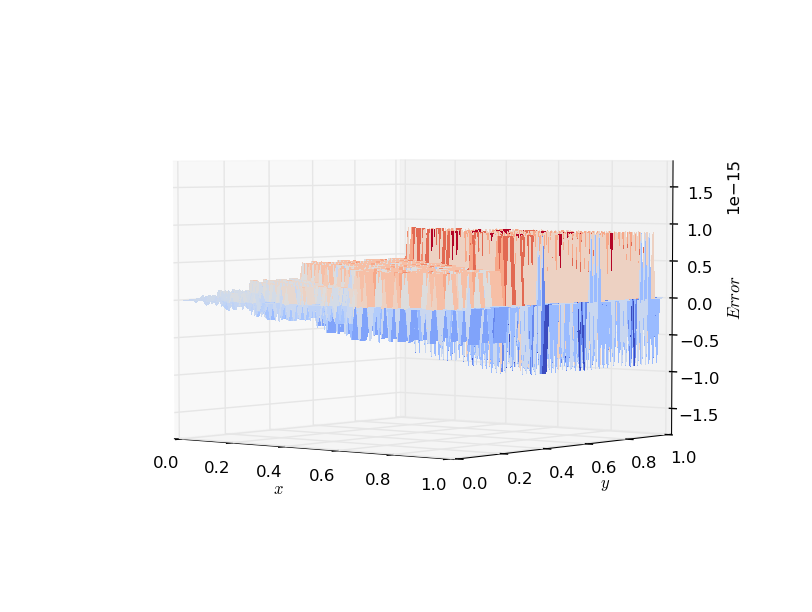
\includegraphics[width=1.0\linewidth]{images/example1_error}
  \caption{Error}
  \label{fig:sub2}
\end{subfigure}
\caption{Analytic (a) and numerical (b) solution for the current Poisson problem, with a surface plot of the  error in (c).}
\label{fig:example1}
\end{figure}

We see that the numerical solution is identical to the analytic one, and the error is shown to be of the order of $10^{-15}$. 

\section{Simple Linear RHS}
Now, we will solve a Poisson problem with a simple linear right-hand-side function. Let us assume that the (known) solution $u(x,y)$ is 

\begin{equation}
u(x,y) = x^2 + y^2
\end{equation}

The corresponding Poisson problem is now

\begin{subequations}
\begin{align}
\nabla ^2 u = &u_{xx} + u_{yy} = 2 + 2 = 4 \\
u(x,0) = x^2 \quad \quad \quad & \quad \quad \quad u(x,y_L) = x^2 + (y_L)^2 \\
u(0,y) = y^2 \quad \quad \quad & \quad \quad \quad u(x_L,y) = (x_L)^2 + y^2
\end{align}
\end{subequations}

We will now solve this Poisson problem and compare the numerical solution with the analytic $(3.4)$.

\subsection{Setting Up The Problem}
We set up the desired Poisson problem, as shown in the previous example, in \emph{setup.c}. Boundary conditions are given by the known solution \emph{(3.4)}, while the RHS function is equal to $4$ for this problem. 
\newline

We set the Boundary Conditions:

\begin{lstlisting}
double fBC(double x, double y) 
{
    return x*x + y*y;
}
\end{lstlisting}

and the RHS function:

\begin{lstlisting}
double f(double x, double y) 
{
    return 4.0;
}
\end{lstlisting}

\subsection{Running the Solver}
We compile the program by typing "make" in the main project directory and run, once again, with 101 grid points in each dimension, as before:
\newline 

\begin{lstlisting}
./poisson2D 101 101
\end{lstlisting}

We produce the surface plot of the results with \emph{visualize.py}. In the next figure, the analytic and numerical solutions are shown side by side for comparison:

\begin{figure}[h!]
\centering
\begin{subfigure}{0.5\textwidth}
  \centering
  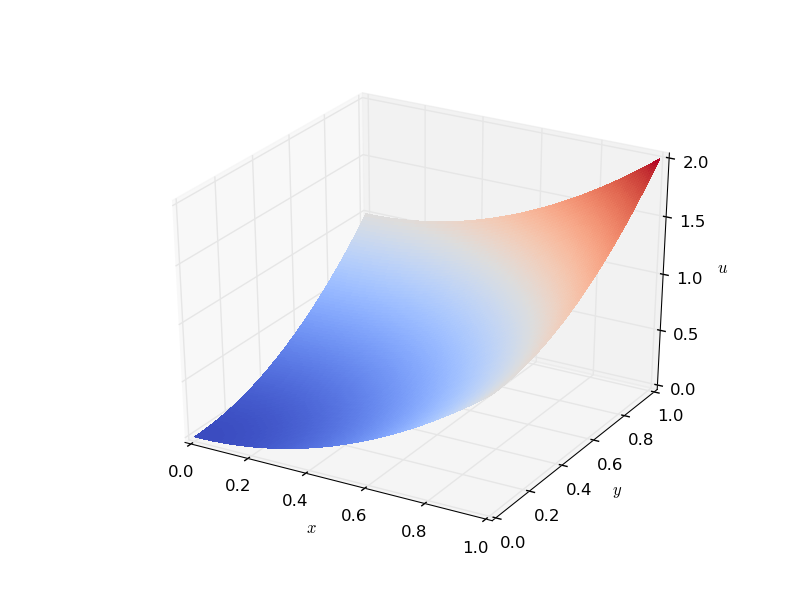
\includegraphics[width=1.0\linewidth]{images/example2_analytic}
  \caption{Analytic solution}
  \label{fig:sub2.1}
\end{subfigure}%
\begin{subfigure}{0.5\textwidth}
  \centering
  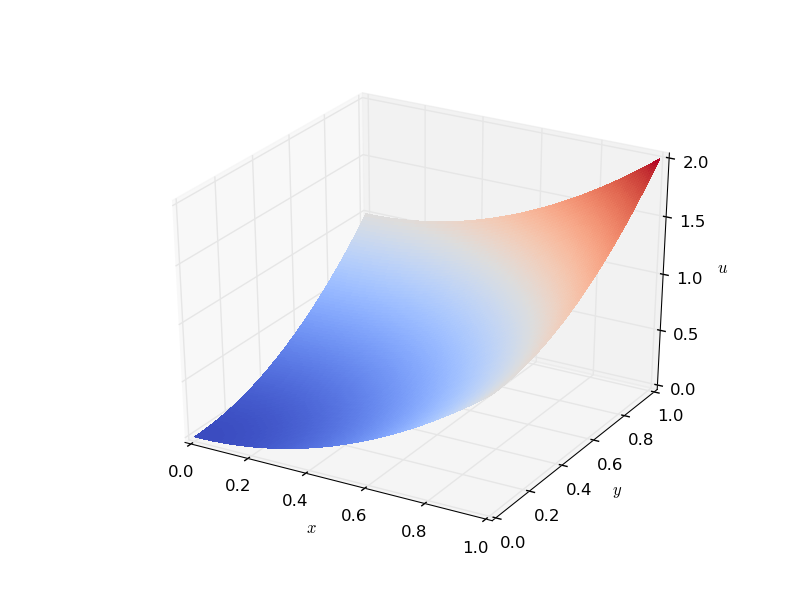
\includegraphics[width=1.0\linewidth]{images/example2_numerical}
  \caption{Numerical solution}
  \label{fig:sub2.2}
\end{subfigure}
\begin{subfigure}{0.6\textwidth}
  \centering
  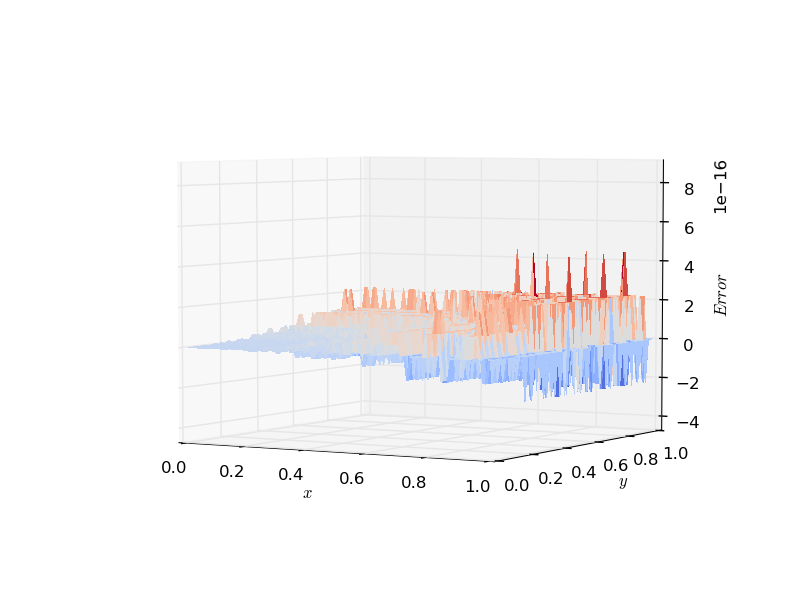
\includegraphics[width=1.0\linewidth]{images/example2_error}
  \caption{Error}
  \label{fig:sub2.3}
\end{subfigure}
\caption{Analytic (a) and numerical (b) solution for the current Poisson problem, with a surface plot of the  error in (c).}
\label{fig:example2}
\end{figure}

We see that the numerical solution is identical to the analytic one, and the error is shown to be of the order of $10^{-16}$. 

\newpage
\section{Sinusoidal RHS}
Now, we will solve a Poisson problem with a slightly more complex right-hand-side function. Let us assume that the (known) solution $u(x,y)$ is 

\begin{equation}
u(x,y) = sin\left[ 2\pi \left( x + y\right) \right]
\end{equation}

The corresponding Poisson problem is now

\begin{subequations}
\begin{align}
\nabla ^2 u = u_{xx} + u_{yy} &= -8\pi^2 sin\left[ 2\pi \left( x + y\right) \right] \\
u(x,0) = sin\left[ 2\pi \left( x \right) \right] \quad \quad & \quad \quad 
u(x,y_L) = sin\left[ 2\pi \left( x + y_L\right) \right]\\
u(0,y) =  sin\left[ 2\pi \left( y \right) \right] \quad \quad & \quad \quad 
u(x_L,y) =  sin\left[ 2\pi \left( x_L + y\right) \right]
\end{align}
\end{subequations}

We will now solve this Poisson problem and compare the numerical solution with the analytic $(3.6)$.

\subsection{Setting Up The Problem}
We set up the desired Poisson problem, as shown in the previous examples, in \emph{setup.c}. Boundary conditions are given by the known solution \emph{(3.6)}, while the RHS function is $f(x,y) =  -8\pi^2 sin\left[ 2\pi \left( x + y\right) \right]$ for this problem. 
\newline

We set the Boundary Conditions:

\begin{lstlisting}
double fBC(double x, double y) 
{
    return sin(2.0*M_PI*(x+y));
}
\end{lstlisting}

and the RHS function:

\begin{lstlisting}
double f(double x, double y) 
{
    return -8.0*M_PI*M_PI*sin(2.0*M_PI*(x+y));
}
\end{lstlisting}

\subsection{Running the Solver}
We compile the program and run with 101 grid points in each dimension, as before:
\newline 

\begin{lstlisting}
./poisson2D 101 101
\end{lstlisting}

We produce the surface plot of the results with \emph{visualize.py}. In the next figure, the analytic and numerical solutions are shown side by side for comparison:

\begin{figure}[h!]
\centering
\begin{subfigure}{0.5\textwidth}
  \centering
  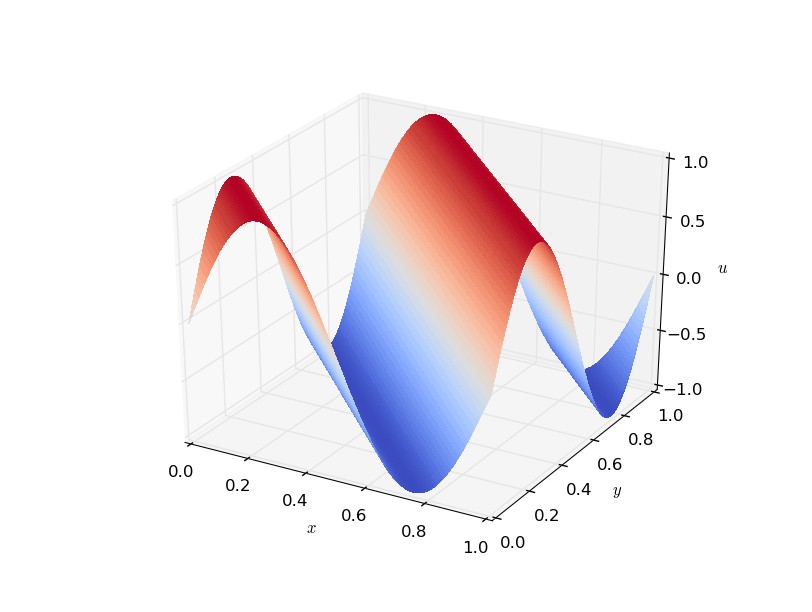
\includegraphics[width=1.0\linewidth]{images/example3_analytic}
  \caption{Analytic solution}
  \label{fig:sub3.1}
\end{subfigure}%
\begin{subfigure}{0.5\textwidth}
  \centering
  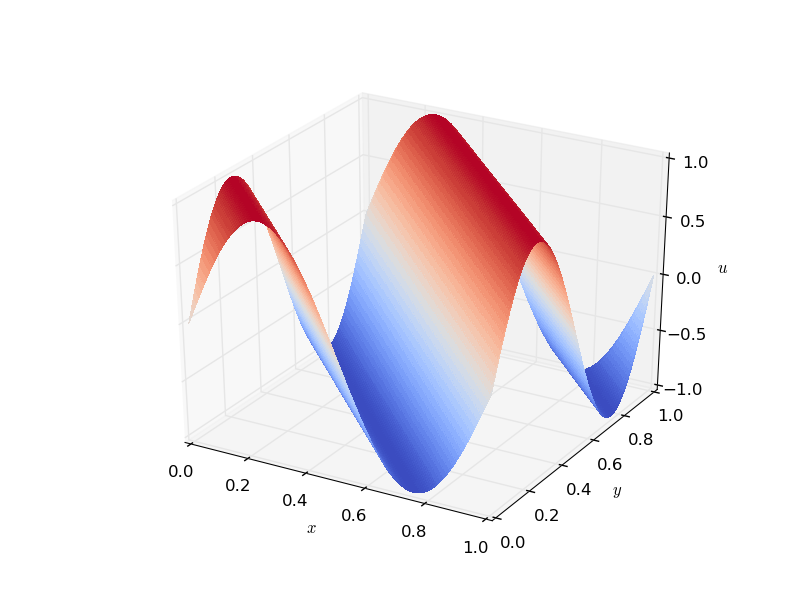
\includegraphics[width=1.0\linewidth]{images/example3_numerical}
  \caption{Numerical solution}
  \label{fig:sub3.2}
\end{subfigure}
\begin{subfigure}{0.6\textwidth}
  \centering
  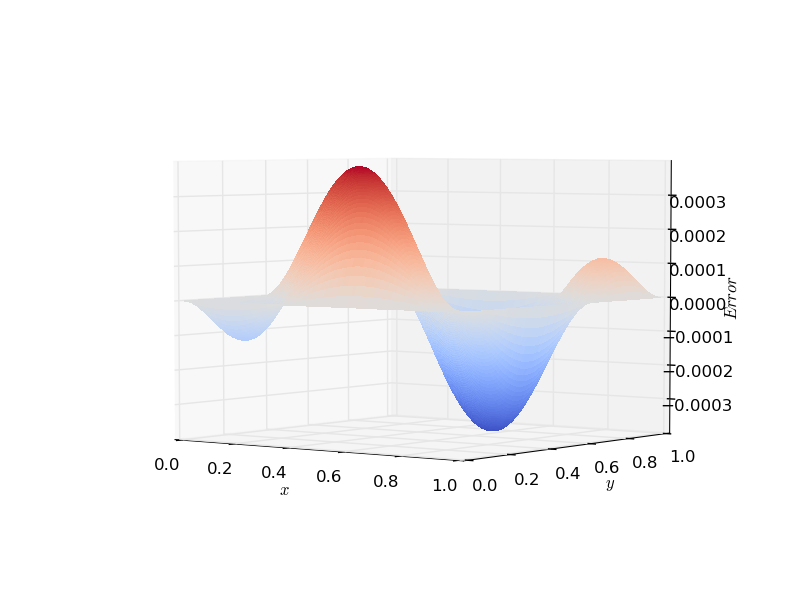
\includegraphics[width=1.0\linewidth]{images/example3_error}
  \caption{Error}
  \label{fig:sub3.3}
\end{subfigure}
\caption{Analytic (a) and numerical (b) solution for the current Poisson problem, with a surface plot of the  error in (c).}
\label{fig:example3}
\end{figure}

We see that the numerical solution is identical to the analytic one, and the error is shown to be of the order of $O(h^2) = O(0.0001)$, where $h = \Delta x = \Delta y = 0.01$. 

\chapter{Performance}
(Under Construction)


\end{document}